\documentclass{article}
\usepackage[utf8]{inputenc}
\usepackage{graphicx}
\usepackage{amssymb}
\usepackage{placeins}
\usepackage{amsmath}
\usepackage{amsthm}
%\usepackage{natbib}
\usepackage{bm}
\def\bhat{\ensuremath{\mathbf{\hat{b}}}}
\def\vpar{\ensuremath{v_{||}}}
\def\vperp{\ensuremath{v_{\perp}}}
\newcommand{\partder}[2]{\dfrac{\partial \, #1}{\partial \, #2}} % partial der.
\newcommand{\der}[2]{\dfrac{d \, #1}{d \, #2}}

\begin{document}

\begin{abstract}

Neoclassical interactions with non-axisymmetric magnetic fields cause a damping force known as neoclassical toroidal viscosity (NTV). The toroidal symmetry of ITER will be broken by the finite number of toroidal field coils and the presence of perturbing ferromagnetic structures such as test blanket modules (TBM) and ferritic inserts (FI). 3D magnetic equilibria are calculated for an ITER steady-state scenario using VMEC, and neoclassical transport quantities in the presence of these error fields are calculated using SFINCS. In the presence of both the FI and TBM, the net effect is a decrease in toroidal damping. The magnitude of NTV torque density at large radii (r/a $\gtrsim$ 0.7) is comparable to the NBI torque density at small radii (r/a $\gtrsim$ 0.4), but is opposite in direction. This could indicate the possibility of generating sheared flows. The magnetic field ripple does not significantly affect the neoclassical tokamak relationship between radial electric field and parallel flow velocity, and at r/a $\gtrsim$ 0.7 the ripple drives additional collisional heat flux comparable to the axisymmetric neoclassical flux.

\end{abstract}

\section{Introduction}

In addition to the magnetic field ripple due to the finite number (18) of toroidal field (TF) coils, the magnetic field in ITER will be perturbed by the addition of ferromagnetic components including ferritic inserts (FIs) and test blanket modules (TBMs). 

TBMs will be installed in three equatorial ports in order to test several tritium breeding concepts and extraction of heat from the blanket. Unfortunately the structural material for these modules is ferritic steel. The TBMs will be installed during the H/He phase in order to test their performance in addition to their possible effects on confinement and transport \cite{Chuyanov2010}. It is important to understand their effect on transport during the early phases of ITER, including their influence on angular momentum transport. Experiments at DIII-D including mock-ups of TBMs indicated a reduction in toroidal rotation by as much as 60\% due to magnetic braking \cite{Schaffer2011}. 

FIs are ferritic steel plates that will be installed at all of the toroidal field coil sections in order to mitigate energetic particle loss due to TF ripple \cite{Tobita2003}. 

In the presence of non-axisymmetric `error fields,' the bounce-averaged radial particle drifts will not necessarily vanish. Several effects can give rise to non-zero radial current: particles trapped poloidally can experience a net radial drift (`banana diffusion'), and particles may become trapped in magnetic wells caused by the perturbing field (`ripple trapping'). As $\nu_{ee} = \sqrt{m_i/m_e} \nu_{ii}$, electrons tend to be in the collision-dominated transport regime in which neoclassical fluxes scale as $1/\nu$.  Therefore ions tend to dominate neoclassical ripple transport, and the resulting particle flux is non-ambipolar. As ambipolarity must be restored for charge conservation, a radial electric field develops to hold the ions back. In a tokamak $v_{\zeta}$ scales with $E_r$; thus a changing radial electric field amounts to a toroidal torque, often referred to as neoclassical toroidal viscosity (NTV). Analytic expressions for neoclassical fluxes in several rippled tokamak transport regimes have been derived, making assumptions about the magnitude of the perturbing field, collisionality, and the collision operator \cite{Shaing2003, Shaing2008, Shaing2010}. 

Indeed, experiments have confirmed the effects of magnetic perturbations on tokamak rotation. 

\section{ITER Steady State Scenario}

\FloatBarrier

\begin{figure}[h!]
\centering
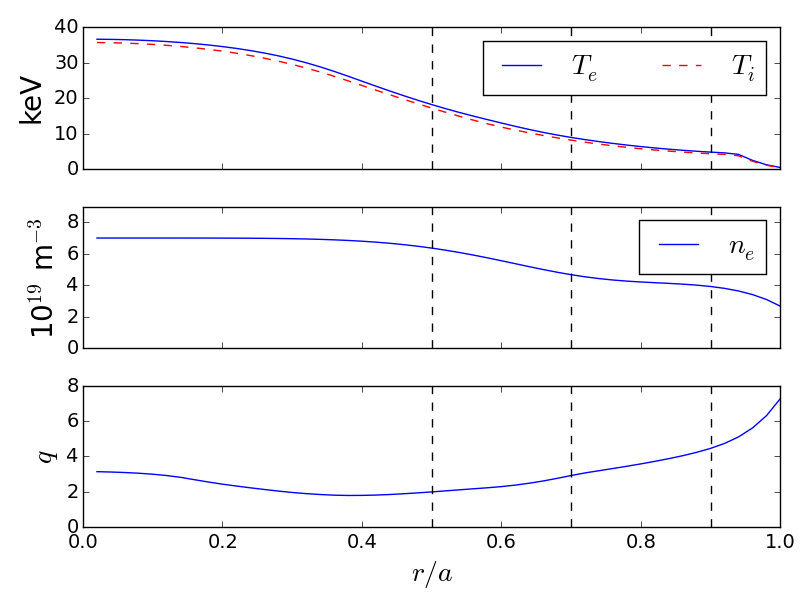
\includegraphics[width=1\textwidth]{profiles.png}
\caption{\label{fig:profiles} Radial profiles of temperature, density, and safety factor for the ITER steady state scenario. Black dashed lines indicate the radial locations that will be considered for neoclassical calculations.}
\end{figure}

VMEC free boundary equilibria and neoclassical transport quantities have been computed for an advanced ITER steady state scenario with significant bootstrap current and reversed magnetic shear \cite{Poli2014}. The input power included 33 MW NBI, 20 MW EC, and 20 MW LH for a fusion gain of $Q = 5$ and toroidal current of 9 MA. The discharge was simulated using the Tokamak Simulation Code (TSC) \cite{Jardin1986} and TRANSP \cite{Hawryluk1980} using a Coppi-Tang transport model and EPED1 \cite{Snyder2011} pedestal modeling. The density, temperature, and safety factor $q$ profiles are shown in figure \ref{fig:profiles}. For neoclassical calculations, impurity species are ignored and it is assumed that $n_D = n_T = n_e$. 

\FloatBarrier

\section{Free Boundary Calculations and Ripple Magnitude}

The magnetic equilibrium was computed using the density, temperature, and $q$ profiles from TRANSP along with filamentary models of the 18 toroidal field (TF) coils and their corresponding currents. The vacuum fields produced by the three TBMs and the FIs have been modeled using FEMAG \cite{Shinohara2009}. The VMEC equilibria is computed using a free boundary model \cite{Hirshman1986} for three cases: (i) including only the toroidal field ripple (ii) including TF ripple, TBMs, and FIs and (iii) including TF ripple and FIs.  

$\delta_B = (B_{max}-B_{min})/(B_{max} + B_{min})$ will be used throughout to quantify the magnitude of ripple, where the maximum and minimum is evaluated at fixed $r_N = \sqrt{\Psi_T/\Psi_T^{LCFS}}$ and $\theta$. In figure \ref{fig:ripplecontour}, $\delta_B$ is plotted on the poloidal plane for the three VMEC equilibria. The components of $B$ with torodial mode number $n = \pm 18$ were removed from the case with TBMs and FIs in order to demonstrate the magnitude of the TBMs alone (bottom right). When only toroidal field ripple is present, significant ripple persists over the entire outboard side, while in the configurations with ferritic inserts the ripple is much more localized in $\theta$. When TBMs and FIs are also present the ripple is higher in magnitude (1.4\%) around the outboard midplane, while in the other magnetic configurations $\delta_B \sim$ 1\% near the outboard midplane. For comparison, the TF ripple during standard operations is $0.08\%$ in JET \cite{DeVries2008} and about $0.6\%$ in ASDEX Upgrade \cite{Martitsch2016}. 

In figure \ref{fig:toroidalripple}, the magnitude of $B$ is plotted as a function of $\zeta$ at $\theta = 0$ and $\theta = \pi/4$. Away from the midplane ($\theta = \pi/4$) the ferritic inserts greatly decrease the magnitude of 18th harmonic of the perturbing field due to the finite number of TF coils. Near the midplane the effect of thee FIs on decreasing the magnitude of this toroidal ripple is much smaller than at $\theta = \pi/4$, as the number of steel plates will be higher away from the midplane \cite{Shinohara2009}. The TBMs add an additional perturbation around $\theta = 0$, as the TBM ports will be located about the midplane. 

\FloatBarrier

\begin{figure}[h!]
\centering
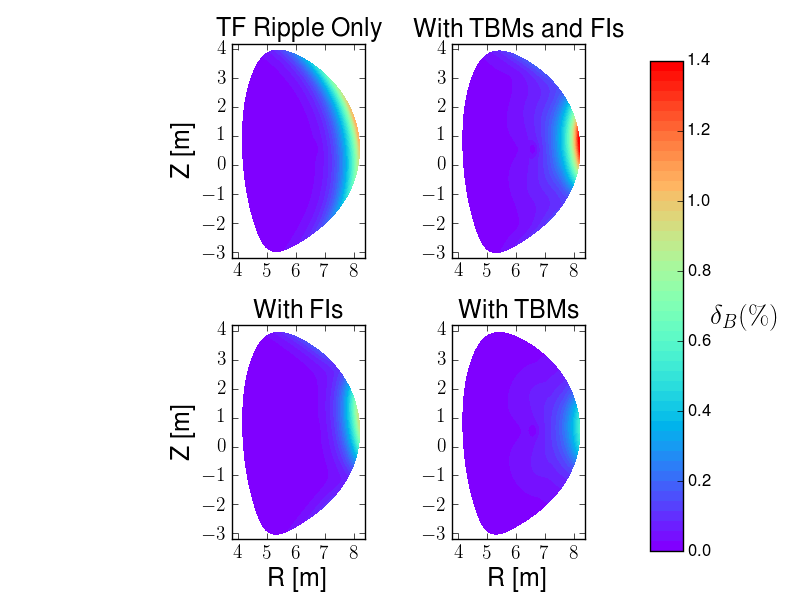
\includegraphics[width=1\textwidth]{ripplecontour.png}
\caption{\label{fig:ripplecontour} $\delta_B = (B_{max}-B_{min})/(B_{max} + B_{min})$ on the poloidal plane for 3 VMEC free boundary equilibria: (i) including only the toroidal field ripple (top left), (ii) including TF ripple, TBMs, and FIs (top right), (iii) including TF ripple and FIs (bottom right), and (iv) with TBMs only.}
\end{figure}

\begin{figure}[h!]
\centering
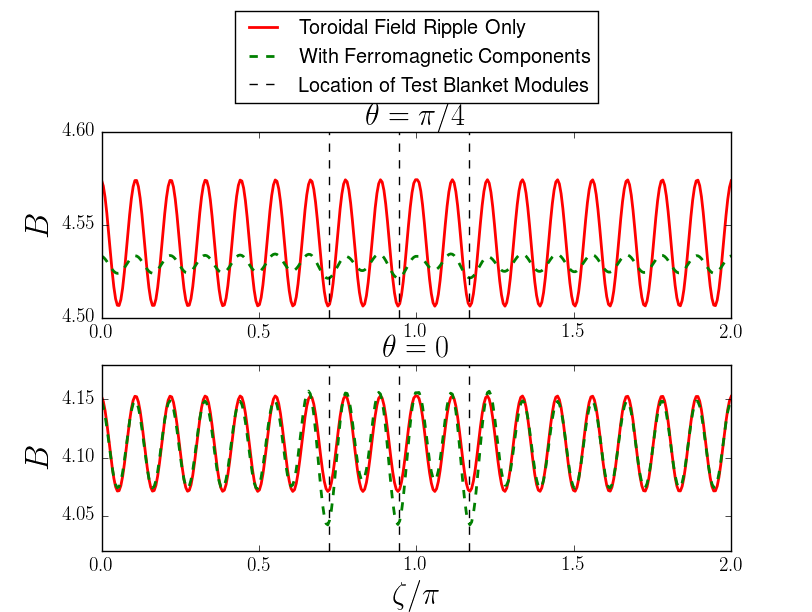
\includegraphics[width=1\textwidth]{toroidalripple.png}
\caption{\label{fig:toroidalripple} The magnitude of $B$ as a function of toroidal toroidal angle ($\zeta$) at $r_N = 1$, $\theta = 0, \pi/4$. Vertical dashed lines indicate the toroidal locations of the TBM ports.}
\end{figure}

\FloatBarrier

\section{Rotation Calculation and Relation to $E_r$}

In order to make predictions of the ripple transport in ITER, the radial electric field, $E_r = - \frac{1}{a} \partder{\Phi}{r_N}$, upon which neoclassical transport depends non-linearly, must first be estimated. This is equivalent to predicting the flow velocity, as $v_{||}$ scales with $E_r$ monotonically. 
As $B_T \gg B_P$, $v_{||} \sim v_{\zeta}$ and the radial electric field can thus be computed from the toroidal rotation. In this calculation of $v_{\zeta}$ the neoclassical torque is ignored: instead $E_r$ is viewed as an input to neoclassical calculations from which the NTV torque can be obtained. 

The following momentum balance equation is considered in determining $v_{\zeta}$
\begin{gather}
\partder{L_{\zeta}}{t} + \nabla \cdot \Pi_{\zeta}^{turb} + \nabla \cdot \Pi_{\zeta}^{NC} = \tau_{NBI}
\end{gather}
where $L_{\zeta}$ is the toroidal angular momentum density, $\Pi^{turb}$ and $\Pi^{NC}$ are the toroidal angular momentum flux density due to turbulence and neoclassical effects, and $\tau_{NBI}$ is the torque density due to NBI. For the moment the neoclassical term will be ignored as this will be calculated as a function of $v_{\zeta}$. $\Pi_{\zeta}^{turb}$ consists of a diffusive term as well as a term independent of $v_{\zeta}$ which accounts for turbulent intrinsic rotation.
\begin{gather}
\Pi_{\zeta}^{turb} = -m_i n_i \chi_{\zeta} R \nabla v_{\zeta} + \Pi_{int}
\end{gather}
Here $R$ is the major radius and $m_i$ and $n_i$ are the ion mass and density. As it is difficult to model the interactions between external torques and intrinsic rotation, these two effects are considered separately in order to generate two estimates for $v_{\zeta}$. For the first model, TRANSP evolves the rotation profiles by balancing turbulent diffusion (assuming $\chi_{\zeta} = \chi_{i}$) and models of neutral beam torques from NUBEAM. 
\begin{gather}
\tau_{NBI} = -m_i n_i \chi_{i} R \nabla v_{\zeta}
\end{gather}
In figure \ref{fig:beamtorque} the total beam torque calculated by NUBEAM including collisional, $\bm{J} \times \bm{B}$, thermalization, and recombination torques \cite{Poli2014} is shown.

% rN = 0.9, T = 0.01
% rN = 0.7, T = 0.02
% rN = 0.5, T = 0.07
\begin{figure}[h!]
\centering
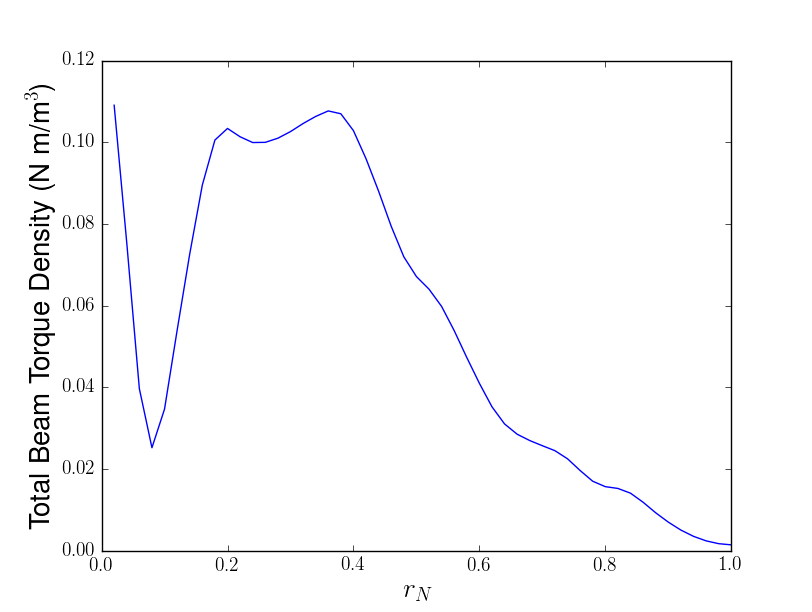
\includegraphics[width=1\textwidth]
{beamtorque.png}
\caption{\label{fig:beamtorque} Total input NBI torque density calculated from NUBEAM.}
\end{figure}

For the second estimate of toroidal rotation a semi-analytic intrinsic rotation model is used \cite{Hillesheim2015}:
\begin{gather}
\Omega_{\zeta}(r_N) = - \int_{r_N}^1 \frac{v_{ti} \rho_{*,\theta}} {2 P_r L_T^2} \widetilde{\Pi} (\nu_*) \, d r'_N,
\end{gather} \label{eq:Hillesheim}
where $v_{ti}$ is the ion thermal velocity, $\rho_{*,\theta} = \frac{v_{ti} m_i}{e B_{\theta}R}$, $P_r = \chi_{\zeta}/\chi_i$ is taken to be 0.7, and $\nu_* = q R v_{ti}/(\nu_{ii} \epsilon^{3/2})$ is the normalized collision frequency. $L_T = - a \left( \partder{\ln T}{r_N} \right)^{-1}$ where $a$ is the minor radius. Expression \ref{eq:Hillesheim} was obtained from assuming that $\Pi_{int}$ balances turbulent momentum diffusion in steady state and that $\Omega_{\zeta} \Pi_{int}/Q \sim \rho_{*, \theta}$, as the rotation is driven by the neoclassical departures from a Maxwellian. It is also assumed that $\Omega_{\zeta} = 0$ at the wall. $\widetilde{\Pi} (\nu_*)$ is an order unity function which characterizes the collisionality dependence of rotation reversals, determined from gyrokinetic turbulence simulations \cite{Barnes2013}. Expression \ref{eq:Hillesheim} was integrated using profiles for the ITER steady state scenario.

The results of these two rotation models are shown In figure \ref{fig:rotation_estimate}. NBI torque contributes to rotation at $r_N \lesssim 0.4$, where the torque density also peaks.  At the radii that will be considered for neoclassical calculations (indicated by dashed vertical lines), rotation due to turbulent momentum redistribution will likely dominate over that due to NBI. Therefore, for the purposes of estimating $E_r$ the intrinsic rotation calculation of $v_{\zeta}$ will be used. The estimated $v_{\zeta}$ from this model is comparable to that predicted from Rice scaling $v_{\zeta} = \Delta W_p/I_P \sim 700$ km/s  ($W_p = 160$ MW, $I_P = 9$ MA). 

\FloatBarrier

% add mach number scale to lower plot
\begin{figure}[h!]
\centering
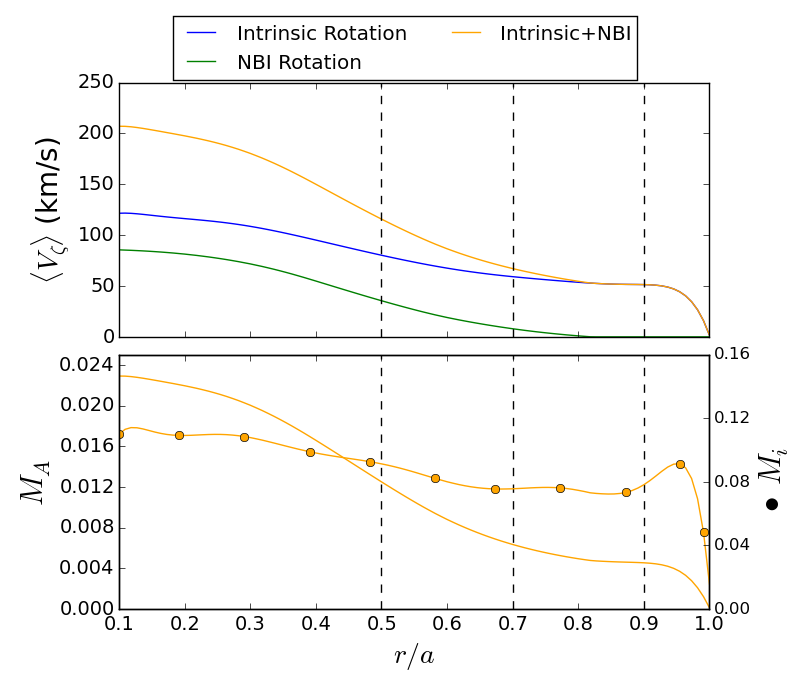
\includegraphics[width=1\textwidth]{rotationestimate.png}
\caption{\label{fig:rotation_estimate} Toroidal rotation $v_{\zeta}$ due to intrinsic rotation and NBI (top), Alfv\`{e}n Mach number  (bottom, solid), and sonic Mach number (bottom, bulleted). Dashed vertical lines indicate the radial positions where SFINCS calculations will be performed. }
\end{figure}

% Discussion of why intrinsic rotation is dominant in ITER
ITER will use a 33 MW NBI system with 1 MeV particle energy to maximize penetration in the core \cite{Poli2014}. For comparison, JET currently uses a 34 MW system with 125 kV particle energy \cite{Ciric2011}. Higher particle energy implies less momentum transport for the same power. While in JET toroidal rotations of up to 700 km/s have been observed \cite{DeVries2008}. Because of ITER's relatively large moment of inertia ($R = 6$ m compared to 3 m for JET), intrinsic rotation will likely be the dominant rotation source. 

For stabilization of the resistive wall mode (RWM) in ITER, it has been estimated that a critical central rotation frequency of about 5\% of the Alfv\`{e}n frequency $\omega_A = B/(R\sqrt{\mu_0 \rho_i})$ must be achieved given a peaked rotation profile. Additionally the TBM are known to increase the critical rotation frequency as they have a much shorter $L/R$ time scale than the wall \cite{Liu2004}. Given the estimated rotation in figure \ref{fig:rotation_estimate} with a central rotation frequency $\omega_0/\omega_A \sim 2\%$, it may be difficult to suppress the RWM in ITER with rotation alone. As this calculation does not take into account magnetic braking, $\omega_0/\omega_A$ will most likely be smaller than what is shown. 

\begin{figure}[h!]
\centering
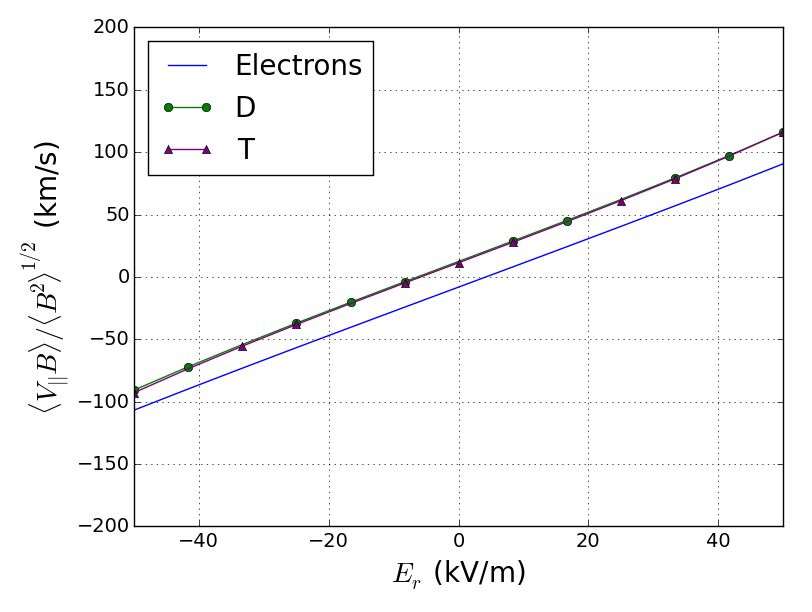
\includegraphics[width=1\textwidth]{Er_flow.png}
\caption{\label{fig:Er_flow} SFINCS calculation of the parallel flow $v_{||}$ at $r_N = 0.9$ for ions and electrons. Results did not change between the calculation with axisymmetric geometry and that with the addition of ripple.}
\end{figure}

Equipped with estimates of $v_{\zeta}$, neoclassical calculations of $v_{||}$ are now made in order to determine the radial electric field $E_r = - \frac{1}{a} \Phi'(r_N)$ . The Stellarator Fokker-Planck Iterative Neoclassical Conservative Solver (SFINCS) \cite{Landreman2014}, is used to solve a radially-local drift kinetic equation with a linearized Fokker-Planck collision operator for the gyro-averaged distribution function on a single flux surface including coupling between species. 
\begin{gather}
( v_{||} \bm{b} + \bm{v}_E + \bm{v}_m) \cdot (\nabla f_{a1})  - C(f_{a1}) = - (\bm{v}_{ma} + \bm{v}_E) \cdot \nabla \psi \left( \partder{f_{a0}}{\psi} \right).
\end{gather} \label{kineticequation}
Transport quantities have been calculated using the steady state scenario ion and electron profiles and VMEC geometry.Calculations will be performed near the edge as this is where ripple is maximized. $E_{||}$ is ignored for this non-inductive scenario.

The relationship between $E_r$ and $v_{||}$ for electrons and ions at $r_N = 0.9$ is shown in figure \ref{fig:Er_flow}. Note that only one curve is shown for each species as the addition of ripple fields did not change the dependence of $v_{||}$ on $E_r$.  

\FloatBarrier

\section{Torque Calculation}

The NTV torque density $\tau_{\zeta}^{NTV}$ is calculated from radial particle fluxes, $\Gamma_{\psi}$, from the flux-friction relation,
\begin{gather}
\tau_{\zeta}^{NTV} = - B^{\theta} \sum_s n_s q_s \Gamma_{\psi},
\end{gather}
where $B^{\theta} = \bm{B} \cdot \nabla \theta$ and the summation is performed over species. 

The calculation of $\tau_{\zeta}^{NTV}$ for three VMEC geometries at $r_N = 0.9$ is shown in figure \ref{fig:Torque_ErandV}. The magnitude of the torque density with only TF ripple is larger than that with the addition of both the FIs and the TBMs. The axisymmetric geometry does not contribute to NTV torque, as expected. The dashed vertical line indicates the value of $v_{||}$ and $E_r$ predicted from the intrinsic rotation model. At this radius for the TF only case, $\tau_{\zeta} = -0.058$ Nm/m$^3$ while for the case with TBMs and FIs it is -0.012 Nm/m$^3$. The circle indicates the `offset rotation' at the ambipolar $E_r$. If no other torques were present in the system, the NTV torque would drive the plasma to rotate at this velocity. Although the $\tau_{\zeta}^{NTV}$ varies significantly between the two geometries they predict similar offset rotation velocities: $v_{\zeta}$ = -10 km/s with TF ripple only and -6 km/s with TBMs and FIs. Note that for $E_r$ greater than this ambipolar value, $\tau_{\zeta}^{NTV}$ is counter-current while neutral beams and turbulence drives rotation in the co-current direction.

With reference to figure \ref{fig:beamtorque}, the NTV torque due to TF ripple only is higher in magnitude than the total beam torque while that with TBMs and FIs is of similar magnitude to the beam torque density. $\tau_{\zeta}^{NTV}$ is also likely to dominate over turbulent torque. Estimating $\Pi_{int} \sim \rho_{*, \theta} Q\, \widetilde{\Pi}/\Omega_{\zeta}$, the magnitude of the torque density due to turbulent momentum redistribution (-$\nabla \cdot \Pi_{int}$) is estimated to be $\lesssim $ 0.01 Nm/m$^3$ at this radius, as the heat flux due to turbulence peaks in the core. Therefore, at these radii $\tau_{\zeta}^{NTV}$ will only have to balance $\tau_{\zeta}^{NBI} = 0.01$ Nm/m$^3$. 

\FloatBarrier

\begin{figure}[h!]
\centering
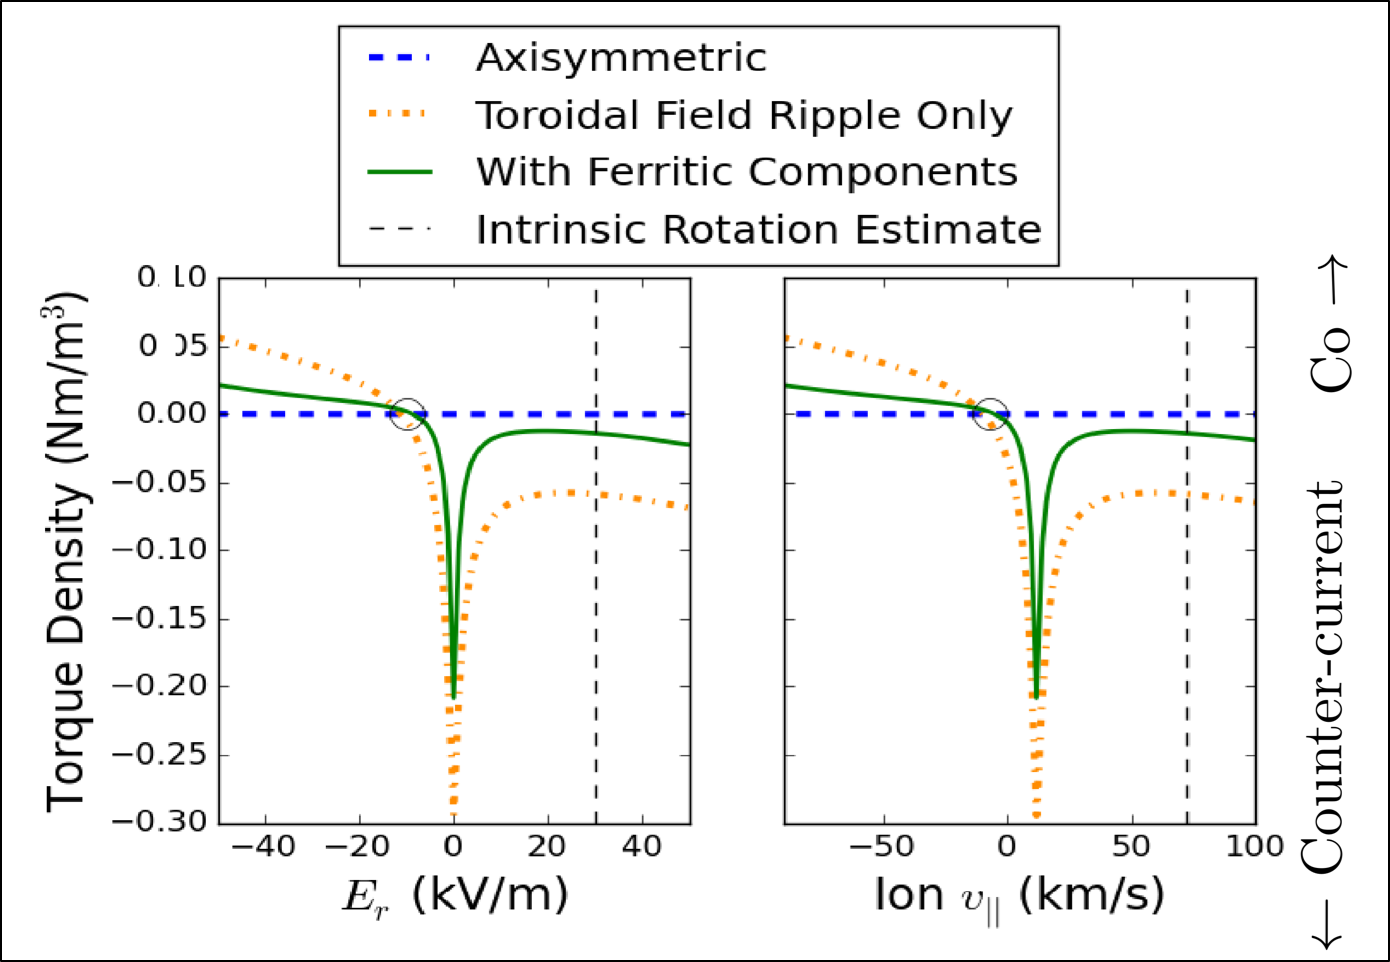
\includegraphics[width=1\textwidth]{Torque_ErandV.png}
\caption{\label{fig:Torque_ErandV} SFINCS calculation of NTV torque density as a function of $E_r$ and $v_{||}$ at $r_N = 0.9$ is shown for 3 VMEC geometries: (i) axisymmettic (blue solid), (ii) with TF ripple only (red dashed), and (iii) TF ripple with FIs and TBMs (red dash-dot). The vertical dashed line indicates the estimate of $E_r$ and $v_{||}$ based on the intrinsic rotation model. The circle denotes the offset rotation at $v_{||} \sim -10$ km/s.}
\end{figure}

In order to decouple the influence of the FI ripple and the TBM ripple, the torque density is calculated at $r_N = 0.9$ for (i) TF ripple with FIs and TBMs, (ii) TF ripple with FIs, and (iii) only TBMs, shown in \ref{fig:Torque_comparingTBMandFI}. The ripple due to the TBMs produce much less $\tau_{\zeta}^{NTV}$ than the TF ripple with the FIs does.  While the FIs decrease the magnitude of the $n = 18$ component of $B$, the TBM contributes to low mode numbers (mostly $n = 1$). In the $\sqrt{\nu}$ regime $\Gamma_{\psi} \sim \sqrt{n}$ and in the $1/\nu$ regime $\Gamma_{\psi} \sim n^2$ \cite{Shaing2010}, so it is reasonable to expect that the higher harmonic ripple of the FIs would increase $\tau_{\zeta}^{NTV}$ more strongly. Moreover, when transport is dominated by the $\bm{E} \times \bm{B}$ precession frequency ($\nu_{eff}/\omega_E \ll 1$), if the poloidal extent of the ripple $\Delta \theta$ is decreased, the characteristic time scale for detrapping $\Delta t \sim \Delta \theta/ \omega_E$ will decrease. If diffusion scales as $D \sim f_t \Delta x^2/\Delta t$, reducing the poloidal extent of ripple will decrease transport. 

\begin{figure}[h!]
\centering
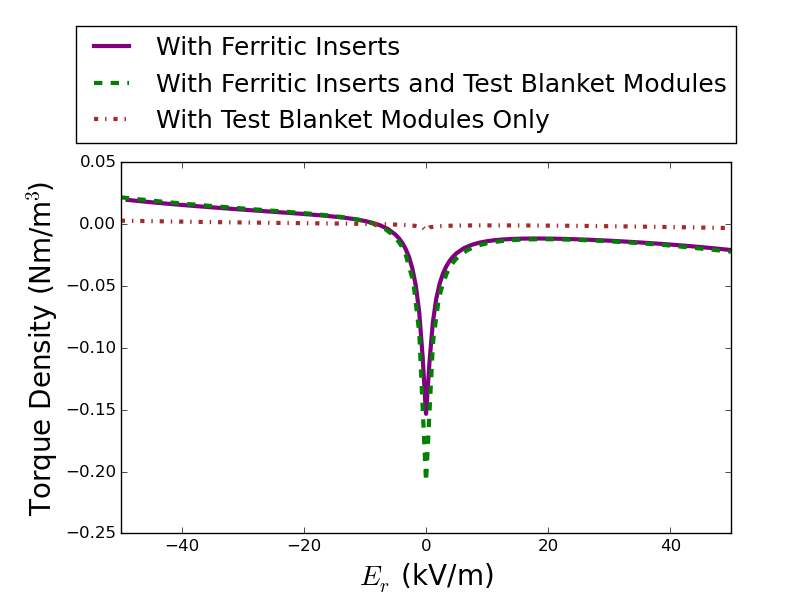
\includegraphics[width=1\textwidth]{Torque_comparingTBMandFI.png}
\caption{\label{fig:Torque_comparingTBMandFI} The NTV torque density at $r_N = 0.9$ for three magnetic geometries: (i) with FIs (purple solid), (ii) with TBMs (brown dash dot), (iii) and with FIs and TBMs (green dashed).}
\end{figure}

In figure \ref{fig:Torque_radiusscaling}, the SFINCS calculation of $\tau_{\zeta}^{NTV}$ with TF ripple only is shown at $r_N$ = 0.5, 0.7, and 0.9. It is expected that the magnitude of transport will decrease with decreasing ripple, as $\Gamma_{\psi} \sim (\delta_B)^2$ in the $1/\nu$ and $\sqrt{\nu}$ regimes and $\sim (\delta_B)$ in the $\nu$ regime. For these three radii the maximum $\delta_B = 0.26\%$, 0.51\%, and 0.82\% respectively. Moreover, the poloidal extent of the ripple decreases with decreasing radius. Indeed, at $r_N \lesssim 0.5$, the neoclassical torque is irrelevant in comparison to the NBI torque (0.6 NM/m$^3$). As the ripple magnitude and poloidal extent peaks at large radius, so will the magnitude of $\tau_{\zeta}^{NBI}$. 

As this significant counter-current torque ($\tau_{\zeta}^{NTV} \lesssim$ - 0.6 NM/m$^3$) peaks at the edge while the NBI torque density ($\lesssim$ 0.1 Nm/m$^3$) peaks at $r_N \sim 0.3$, there may be a possibility of generating sheared rotation. If neoclassical effects dominate at the edge, based on the offset rotation with TF ripple with TBMs and FIs, $v_{\zeta}$ = -6 km/s at $r_N = 0.9$. 

% Extend V_|| scan up to 150 km/s so matches up with horizontal line estimates
\begin{figure}[h!]
\centering
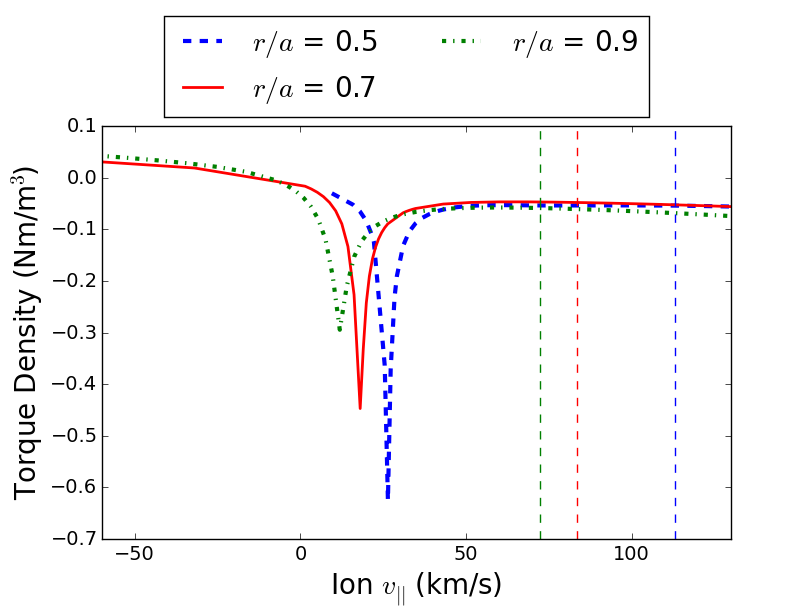
\includegraphics[width=1\textwidth]
{Torque_radiusscaling.png}
\caption{\label{fig:Torque_radiusscaling} SFINCS calculation of NTV torque density ($\tau_{\zeta}^{NTV}$) as a function of ion $v_{||}$ for VMEC geometry with TF ripple only at $r_N$ = 0.5 (blue solid), 0.7 (red dashed), and 0.9 (green dash-dot).}
\end{figure}

% I should redo this scan with Er = 30


\FloatBarrier

\section{Scaling with Ripple Magnitude}
The scaling of NTV transport with the magnitude of $\delta_B$ shows some agreement with that predicted by Shaing \cite{Shaing2008}. In figure \ref{fig:scalescan}, the NTV torque density calculated by SFINCS is shown as a function of the magnitude of the TF ripple, $\delta_B$. The additional ferromagnetic ripple is not included, while the $n=18$ component of $B$ is rescaled. $\tau^{NTV}$ is calculated at $r_N = 0.9$ with $E_r = 30$, corresponding to the intrinsic rotation estimate. The color-shaded background indicates the approximate regions of applicability of the $\sqrt{\nu}$ and $\nu$ regimes. The $1/\nu$ regime does not apply as $\omega_E \gg \nu/\epsilon$, where $\omega_E = \frac{E_r}{B}$. 

In the collisional boundary layer, neoclassical fluxes scale as $\sqrt{\nu}$. This regime becomes relevant when the poloidal $\bm{E} \times \bm{B}$ precession frequency is larger than the effective collision frequency of detrapping banana particles, $\nu/\epsilon < \omega_E$, and the ripple magnitude is not large enough for collisionless detrapping to take effect, $\delta_B < \left( \frac{ \epsilon \nu}{\omega_E} \right)^{1/2}$ \cite{Shaing2008}. 
% discussion of collisionless retrapng - trapping regime in Kasilov (42)
In the collisionless trapping-retrapping regime, neoclassical fluxes scale with $\nu$. This regime becomes relevant when $\delta_B > \left( \frac{ \epsilon \nu}{\omega_E} \right)^{1/2}$, i.e. the perturbing field becomes large enough that poloidally trapped particles can become detrapped and retrapped by the ripple \cite{Shaing2010}. In the $\sqrt{\nu}$ regime $\tau_{\zeta}^{NTV} \sim \delta_B^2$ and in the $\nu$ regime $\sim \delta_B$. As $\delta_B$ nears the boundary between the $\sqrt{\nu}$ and $\nu$ regimes, the scaling of $\tau_{\zeta}^{NTV}$ with $\delta_B$ becomes shallower until it approaches the scaling expected. When $\delta_B \sim \epsilon$, the poloidal field variation no longer becomes the dominant perturbation. The departure of numerical results from predicted scaling can be attributed to the model whch bounce-averaging of the kinetic equation and assumption of large aspect ratio. 

\begin{figure}[h!]
\centering
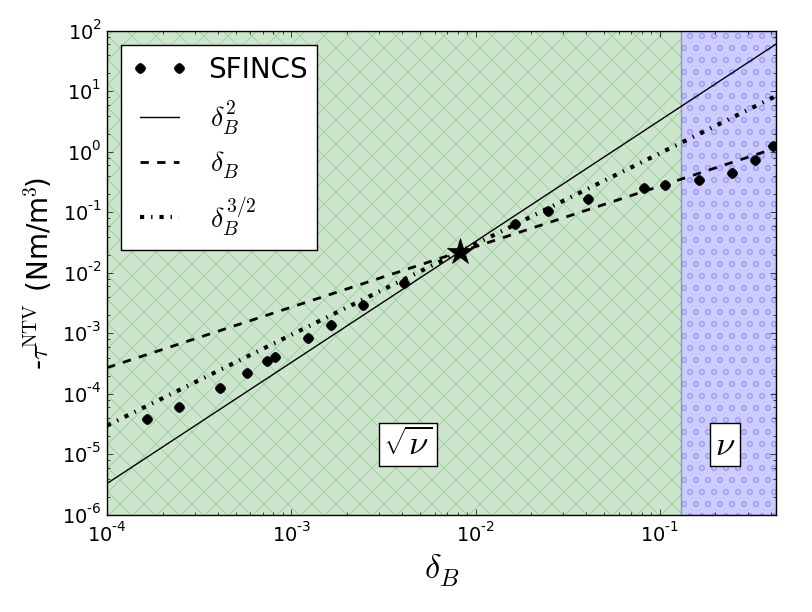
\includegraphics[width=1\textwidth]
{scalescan.png}
\caption{\label{fig:scalescan} SFINCS calculations of NTV torque density as a function of $\delta_B$ at $r_N = 0.9$. A single value of $E_r$ is used corresponding to the intrinsic rotation estimate. Color-shaded area indicates the approximate regions of applicability for rippled tokamak regimes.}
\end{figure}

\FloatBarrier

\section{Heat Flux Calculation}

In addition to driving non-ambipolar particle fluxes, the breaking of toroidal symmetry drives additional neoclassical heat flux. In figure \ref{fig:HeatFlux}, the SFINCS calculation of heat flux is shown for three magnetic geometries: (i) axisymmetric (blue solid), (ii) with TF ripple only (green dashed), and (iii) TF ripple with TBMs and FIs (red dash-dot). In the presence of TF ripple, the additional heat flux is comparable to the axisymmetric case. However, with the addition of the FIs the heat flux is reduced to the magnitude of the axisymmetric value, except near $E_r = 0$ where $1/\nu$ transport dominates. 

While the radial ripple-drive particle fluxes will significantly alter the ITER angular momentum transport, it should be noted that the neoclassical particle fluxes are insignificant in comparison to the turbulent heat flux, which will amount to $\sim 0.05$ MW/m$^2$ at the radii under consideration. If ITER ripple were scaled up to $\delta_B \gtrsim 50\%$, the neoclassical ripple heat transport would be comparable to the anomalous transport.

\begin{figure}[h!]
\centering
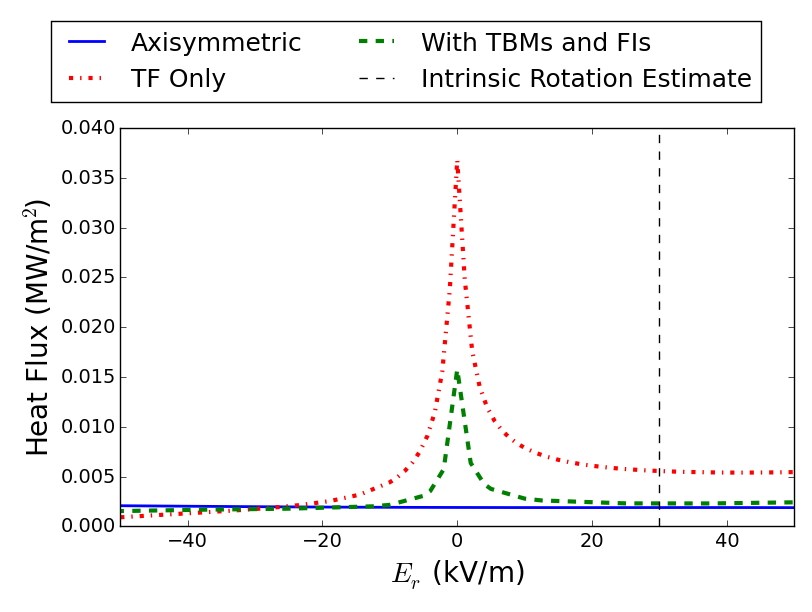
\includegraphics[width=1\textwidth]
{HeatFlux.png}
\caption{\label{fig:HeatFlux} SFINCS calculation of neoclassical heat flux for three magnetic geometries: (i) axisymmetric (blue solid), (II) with TF ripple only (green dashed), and (iii) TF ripple with TBMs and FIs (red dash-dot).}
\end{figure}

\FloatBarrier

\section{Radially Local Approximation of Magnetic Drifts}
Although $(v_E + \bm{v}_m) \cdot \nabla f_1$ is formally of lower order than the other terms in \ref{kineticequation}, it has been found to be important when $\rho_* \sim \nu_*$ and has been included in other calculations of 3D neoclassical transport. In the calculations shown above this term has not been included. 
 As SFINCS does not maintain radial coupling of $f_1$, there are several radially-local models of toroidal and poloidal $\bm{v}_d$.  The Kasilov form ((67) in \cite{Kasilov2014}) ignores the toroidally varying components of $\bm{B}$ and the radial variation of $q$. The Martitsch form ((16) in \cite{Martitsch2016}) is the same as the Kasilov form but maintains magnetic shear dependence. This non-local effect has been shown to be important in NTV transport regimes \cite{Martitsch2016}. The Sugama form is obtained by subtracting off the radial component of $\bm{v}_m$ and multiplying by a factor which ensures that $\bm{v}_m (\mu = 0)  = 0$ in order to remove sources/sinks in velocity space. Each of these magnetic drift schemes are independent of the choice of Boozer angle. 

An $E_r$ scan at $r_N = 0.9$ is shown in figure \ref{driftschemes}. When $\bm{v}_m$ is added to the kinetic equation, the $1/\nu$ valley is shifted toward a slightly negative $E_r$, corresponding to the region where $\omega_E + \omega_M = 0$. However, the addition of $v_m \cdot \nabla f_1$ has a negligible effect on transport at the edge. 

\begin{figure}[h!]
\centering
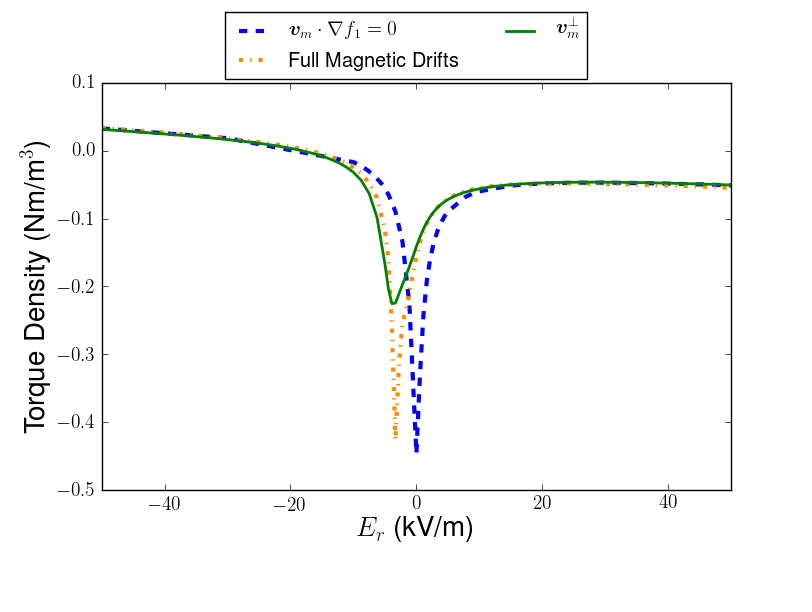
\includegraphics[width=1\textwidth]{mdscomparison.png}
\caption{Comparison of magnetic drift models at $r_n = 0.9$. NTV torque density is calculated for the ITER steady state scenario as a function of $E_r$. }
\end{figure}\label{driftschemes}

\bibliographystyle{abbrv}
\bibliography{ITERNTV}

\end{document}
